%
% main.tex -- Paper zum Thema <logistic>
%
% (c) 2020 Hochschule Rapperswil
%
\chapter{Iteration der logistischen Gleichung\label{chapter:logistic}}
\lhead{Logistische Gleichung}
\begin{refsection}
\chapterauthor{Michael Arthur Schneeberger}
\index{Schneeberger, Michael Arthur}%
\index{logistische Gleichung}%

%\renewcommand{\floatpagefraction}{0.5}

%
% einleitung.tex -- Beispiel-File für die Einleitung
%
% (c) 2020 Prof Dr Andreas Müller, Hochschule Rapperswil
%
\section{Modellierung von Populationen
\label{logistic:section:einleitung}}
\rhead{Modellierung von Populationen}

Die logistische Gleichung ist ein beliebtes mathematisches Objekt,
das zeigt, wie aus einer scheinbar einfach Gleichung
ein sehr komplexes und chaotisches Verhalten entstehen kann. 
\index{chaotisch}%
Ihren Urpsrung hat die logistische Gleichung beim Modellieren
vom zeitlichen Verlauf von Populationen. 
\index{Population}%
Wie man dabei ganz organisch auf die logistische Gleichung 
kommt, wird in diesem Abschnitt kurz demonstriert. 
\index{logistische Gleichung}%

Als Erstes nehmen wir eine Population an, 
die ungehindert wachsen kann. 
Anfänglich hat diese die Tendenz, exponentiell zu wachsen. 
\index{exponentielles Wachstum}%
Sei $x_{n}$ die Population zu einem bestimmten Zeitpunkt, 
beispielsweise am Anfang vom Jahr $n$. 
Nun ist $x_{n+1}$ die Population im darauf folgenden Jahr, 
welche eine direkte Funktion der Population im vorherigen
Jahr ist. 
Ein einfaches mathematisches Modell für dieses Verhalten
könnte wie folgt aussehen:
\begin{equation}
    \label{eq:lambda_xn}
    x_{n+1} = \lambda x_{n}\text{.}
\end{equation}
Der Faktor $\lambda$ gibt in diesem Modell an, 
wie schnell die Population von Jahr zu Jahr ansteigt. 
Es ist schnell erkennbar, 
dass ein $\lambda > 1$ ein Wachstum und
ein $\lambda < 1$ einen Zerfall
der Population im folgenden Jahr zur Folge hat. 
Abbildung \ref{fig:pop_exp} zeigt die jährlichen
Entwicklungen von Populationen für verschiedene
Werte von $\lambda$ mit diesem Modell.
Auf der linken Grafik mit $\lambda = 0.75$ ist deutlich
ein exponentieller Zerfall und auf 
der rechten Grafik mit $\lambda = 1.25$
ein exponentielles Wachstum ersichtlich.
\begin{figure}
    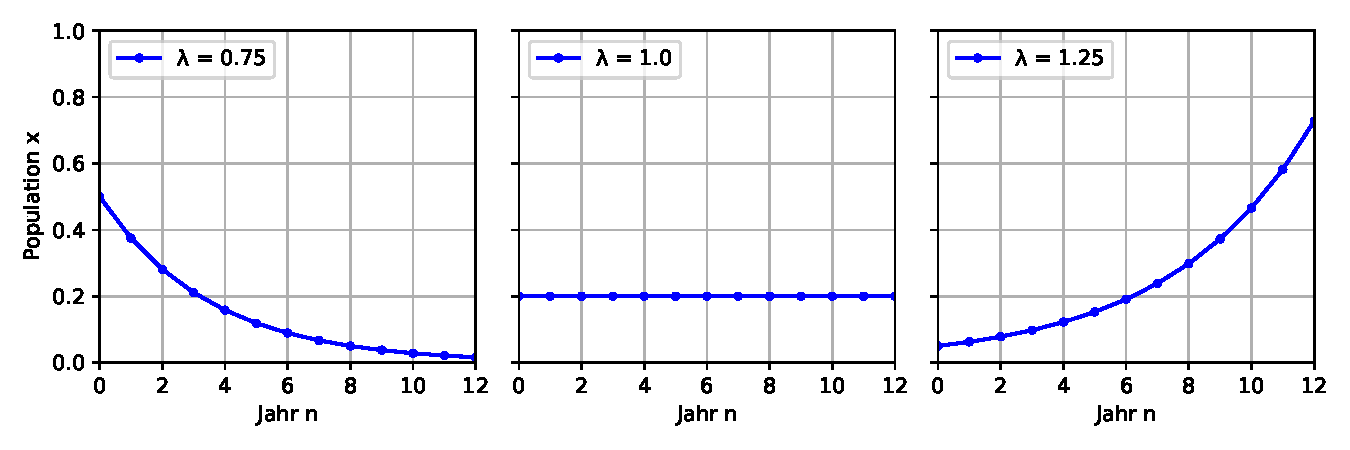
\includegraphics[width=\linewidth]{papers/logistic/figures/pop_exp.pdf}
    \caption{
        Exponentielle Populationsverläufe nach
        Gleichung \eqref{eq:lambda_xn}
        und verschiedenen Werten von $\lambda$.
    }
    \label{fig:pop_exp}
\end{figure}

In der Realität können Populationen natürlich nicht endlos
exponentiell weiterwachsen, 
da früher oder später Platz, Nahrung, usw. ausgehen.
Um dieses Verhalten in das Modell zu implementieren,
fügen wir noch einen zusätzlichen Term hinzu, 
womit wir auch schon bei der logistischen Gleichung 
\begin{equation}
    \label{eq:logistic}
    x_{n+1} = \lambda x_{n} (1 - x_{n})
\end{equation}
angekommen sind.
Dieser neue Term sorgt dafür, 
dass das Wachstum der Population zurückgeht, 
wenn sie grösser wird.
Der Wert von $x_n$ ist so limitiert auf 
$0 \le x_n \le 1$  
und kann als die relative Population mit einem
theoretischen Maximum von 1 interpretiert werden. 
Abbildung \ref{fig:pop_logistic} zeigt nun
für einige Werte von $\lambda$\
die jährlichen Entwicklungen von Populationen 
welche mit der logistischen Gleichung modelliert werden.
Dazu ist zum Vergleich das bereits bekannte exponentielle Modell
mit gleichem $\lambda$ als gestrichelte Linie abgebildet. 
Auf der linken Grafik ist auch hier wieder erkennbar, 
dass ein $\lambda < 1$ zur Folge hat, 
dass die Population rasch ausstirbt. 
Auf der mittleren Grafik mit $\lambda = 1.8$ sieht 
die Kurve zuerst annähernd exponentiell wachsend aus,
doch der neu hinzugefügte Term sorgt jetzt dafür, 
dass das Wachstum bei grösser werdender Population zurückgeht 
und sich schliesslich auf $\approx 0.42$ einpendelt. 
Sehr interessant ist die rechten Grafik mit $\lambda = 2.8$,
wo die Population zuerst ein wenig ``überschwingt'', 
sich aber schliesslich auf $\approx 0.62$ einpendelt.  
\begin{figure}
    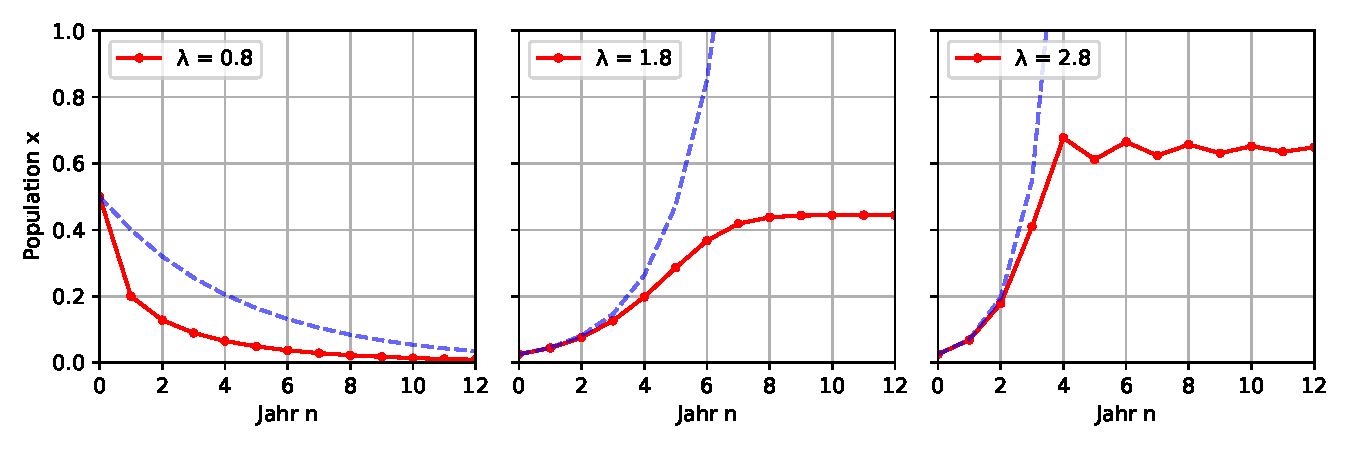
\includegraphics[width=\linewidth]{papers/logistic/figures/pop_logistic.pdf}
    \caption{
        In rot:
        logistische Populationsverläufe nach
        Gleichung \eqref{eq:logistic} und
        verschiedenen Werten von $\lambda$.
        In blau, zum Vergleich:
        exponentielle Populationsverläufe nach 
        Gleichung \eqref{eq:lambda_xn} mit gleichem $\lambda$.
    }
    \label{fig:pop_logistic}
\end{figure}

%
% problemstellung.tex -- Beispiel-File für die Beschreibung des Problems
%
% (c) 2020 Prof Dr Andreas Müller, Hochschule Rapperswil
%
\section{Iteration der logistischen Gleichung
\label{logistic:section:analyse}}
\rhead{Iteration der logistischen Gleichung}

Im Abschnitt \ref{buch:section:iteration} haben wir uns
bereits mit dem Iterieren von Funktionen befasst. 
Genau dieses Prinzip der Iteration finden wir auch bei
der logistischen Gleichung wieder. 
Jede Berechnung der Population im Folgejahr ist 
eine Iteration der logistische Gleichung.
Die logistische Gleichung \eqref{eq:logistic} könnte man 
auch als Funktion $f(x) = \lambda x(1-x)$ schreiben.
Jede Iteration ist nun eine Verschachtelung von $f(x)$,
somit lässt sich jeder beliebige Wert $x_n$ auch wie folgt berechnen:  
\begin{itemize}
    \item $x_1 = f(x_0)$
    \item $x_2 = f(x_1) = f(f(x_0))$
    \item $x_3 = f(x_2) = f(f(f(x_0)))$
    \item $x_4 = f(x_3) = f(f(f(f(x_0))))$
    \item $x_5 = ...$
\end{itemize}

Wir haben im Kapitel 
\ref{logistic:section:einleitung} 
bereits beobachtet,
dass die logistische Gleichung beim Iterieren für 
verschiedene Werte von $\lambda$ gegen verschiedene 
Endwerte konvergiert. 
Der Anfangswert $x_0$ scheint dabei keine Rolle zu spielen
solange er sich im Bereich $0 < x < 1$ befindet, 
er beinflusst lediglich die Form der Kurve, 
bevor sie den Konvergenzwert erreicht. 
Das heisst, wir können $x_0$ einfach auf einen bestimmten Wert, 
zum Beispiel 0.1, setzen. 
Nun können wir $\lambda$ ebenfalls auf einen bestimmten Wert setzen
und die logistische Gleichung endlos iterieren, 
um zu sehen, gegen welchen Wert $x_n$ schliesslich konvergiert.
Mit dem Computer können natürlich nicht unendlich viele Iterationen
durchgeführt werden, aber wenn $n$ gross genug ist, 
kommt man doch sehr nahe an den tatsächlichen Konvergenzwert. 
Genau dieser Prozess ist nun in Abbildung \ref{fig:map_1} 
ersichtlich. 
Sie zeigt einen Plot, 
auf dem die horizontale Achse die verschiedenen Werte
von $\lambda$ im Bereich für $0 \leq \lambda \leq 4$ annimmt 
und die vertikale Achse anzeigt,
auf welchem Wert $x_n$ konvergiert, wenn $n$ gegen
unendlich läuft. Dabei werden einige Eigenschafen 
von der Iteration der logistischen Gleichung ersichtlich:
\begin{figure}
    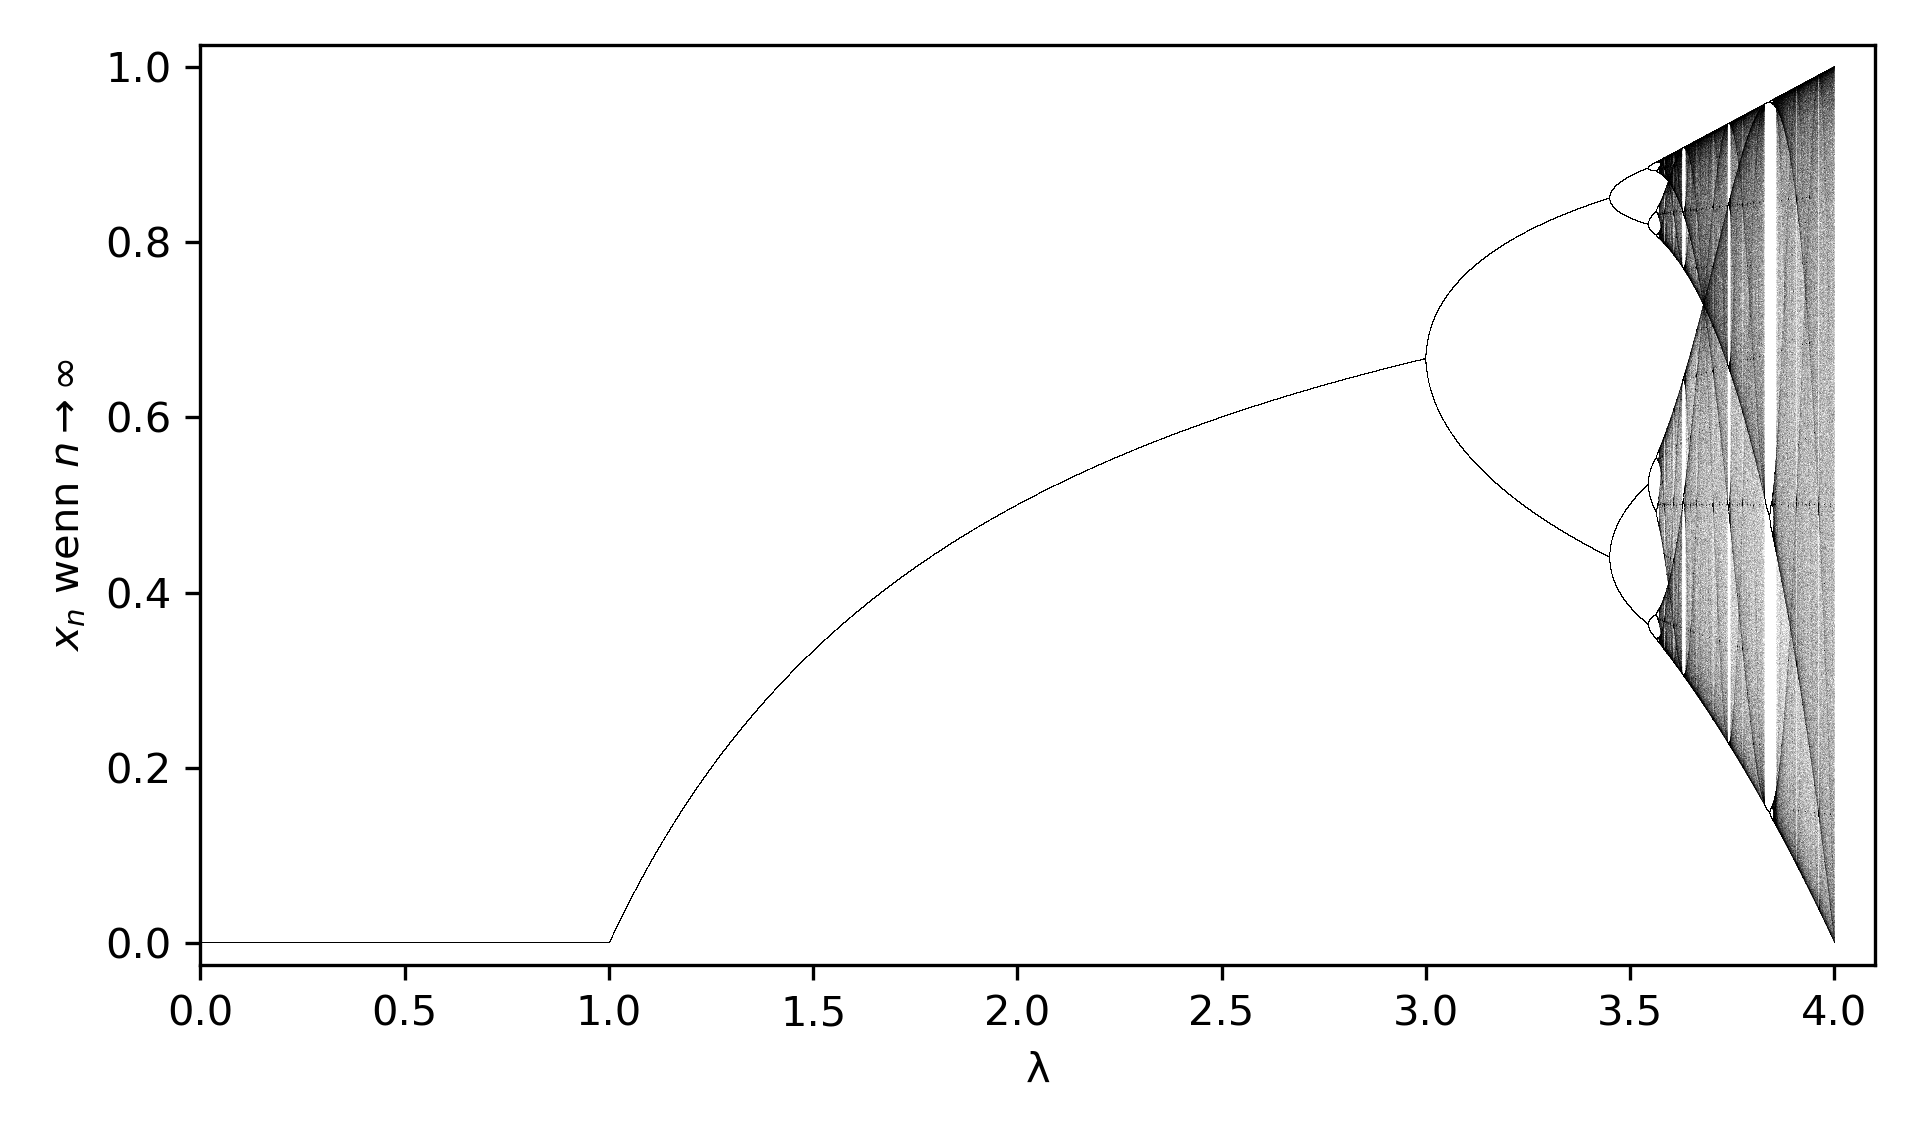
\includegraphics[width=\linewidth]{papers/logistic/figures/map.png}
    \caption{
        Bifurkationsdiagramm der logistischen Gleichung \eqref{eq:logistic}.
        Das Diagramm zeigt für jeden Wert von $\lambda$
        welche Werte $x_n$ annimmt wenn $n \rightarrow \infty$.
    }
    \label{fig:map_1}
\end{figure}
\begin{itemize}
    \item 
    für $0 \le \lambda \le 1$ konvergiert $x_n$ gegen 0
    \item 
    für $1 \le \lambda \le 3$ konvergiert $x_n$ gegen einen fixen Wert
    \item 
    für $3 \le \lambda \le 4$ scheint $x_n$ nicht mehr gegen einen fixen Wert zu konvergieren.
    Stattdessen gibt es diese Verzweigungen, 
\index{Verzweigung}%
    die darauf hindeuten, 
    dass $x_n$ zuerst bis $\lambda \approx 3.4$ zwischen zwei Werten hin und her oszilliert, 
    dann bis $\lambda \approx 3.6$ zwischen vier Werten, dann 8, 16, usw. 
    Dieses Phänomen wird auch ``Periodenverdoppelung'' genannt.
\index{Periodenverdoppelung}%
    \item
    für $\lambda > 4$ gibt es scheinbar nichts mehr.
    Das kommt daher, dass $x_n$ ab da nur noch divergiert.  
\end{itemize}
\begin{figure}
    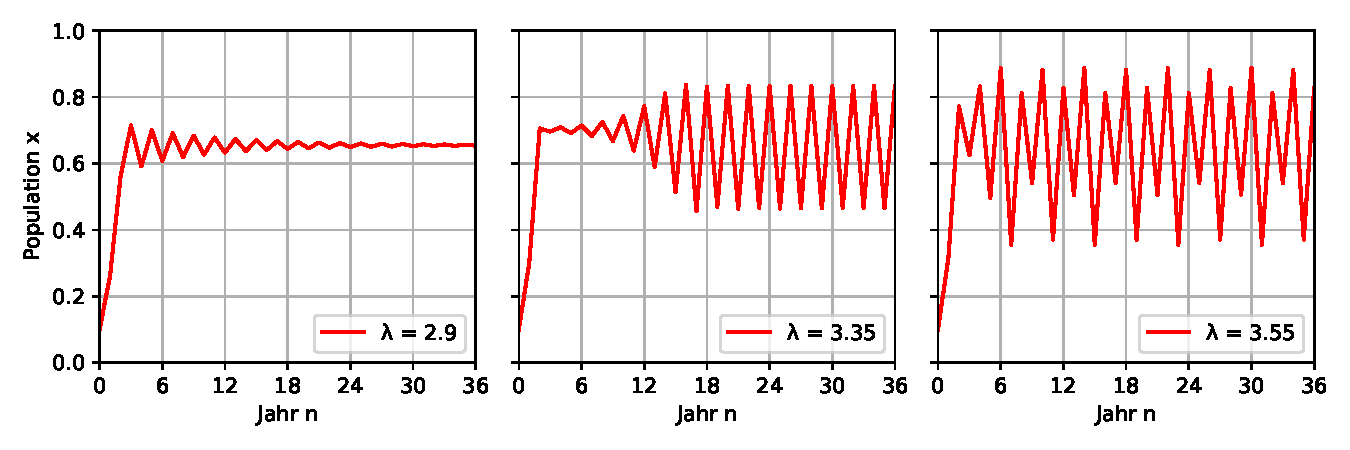
\includegraphics[width=\linewidth]{papers/logistic/figures/pop_logistic_2.pdf}
    \caption{
        Iteration der logistischen Gleichung. 
        Für $\lambda = 2.9$ konvergiert $x_n$ gegen
        $\approx 0.62$.
        Im Kontrast dazu oszilliert $x_n$ für
        $\lambda = 3.35$ und zwischen zwei 
        und für
        $\lambda = 3.55$ sogar zwischen vier Werten. 
    }
    \label{fig:pop_logistic_2}
\end{figure}
Das doch eher spezielle Verhalten von $3 < \lambda < 4$ wird 
auch in Abbildung \ref{fig:pop_logistic_2} ersichtlich,
wenn man die Werte der einzelnen Iteration plottet.
Im ersten Plot mit $\lambda = 2.9$ sieht man, dass $x_n$ zuerst oszilliert,
aber schliesslich auf einen fixen Wert konvergiert.
Auf dem zweiten Plot mit $\lambda = 3.35$ scheint $x_n$ 
nach einigen Iterationen nur noch
zwischen zwei Werten zu oszillieren und beim
dritten Plot mit $\lambda = 3.55$ sogar zwischen vier Werten. 
Dieses Oszillieren zeigt sich in Abbildung \ref{fig:map_1}
durch die Verzweigungen oder auch ``Bifurkationen''. 
\index{Bifurkation}%
\index{Bifurkationsdiagramm}%
Darum wird sie auch ``Bifurkationsdiagramm'' genannt. 

Auf dem Bifurkationsdiagramm sind noch mehr 
interessante Eigenschaften der logistischen Gleichung erkennbar.
Wenn wir, wie in Abbildung \ref{fig:map_zoom}, in die Bereiche hineinzoomen
wo die Bifurkationen immer dichter werden, finden wir Gebilde, 
welche wieder fast genau gleich aussehen.
Tatsächlich könnte man endlos immer weiter in diese
Bereiche hineinzoomen und würde immer wieder auf solche änhlichen Muster stossen. 
Diese Selbstähnlichkeit ist eine typische Eigenschaft von Fraktalen.
\index{Selbstähnlichkeit}%
\index{Fraktal}%
Das Bifurkationsdiagramm der logistischen Gleichung ist also ein Fraktal.
Es gibt sogar einen Zusammenhang zwischen der logistischen Gleichung und 
einem anderen berühmten Fraktal, der Mandelbrotmenge.
\index{Mandelbrotmenge}%
Mehr dazu später in Abschnitt 
\ref{logistic:section:beispiele}.
\begin{figure}
    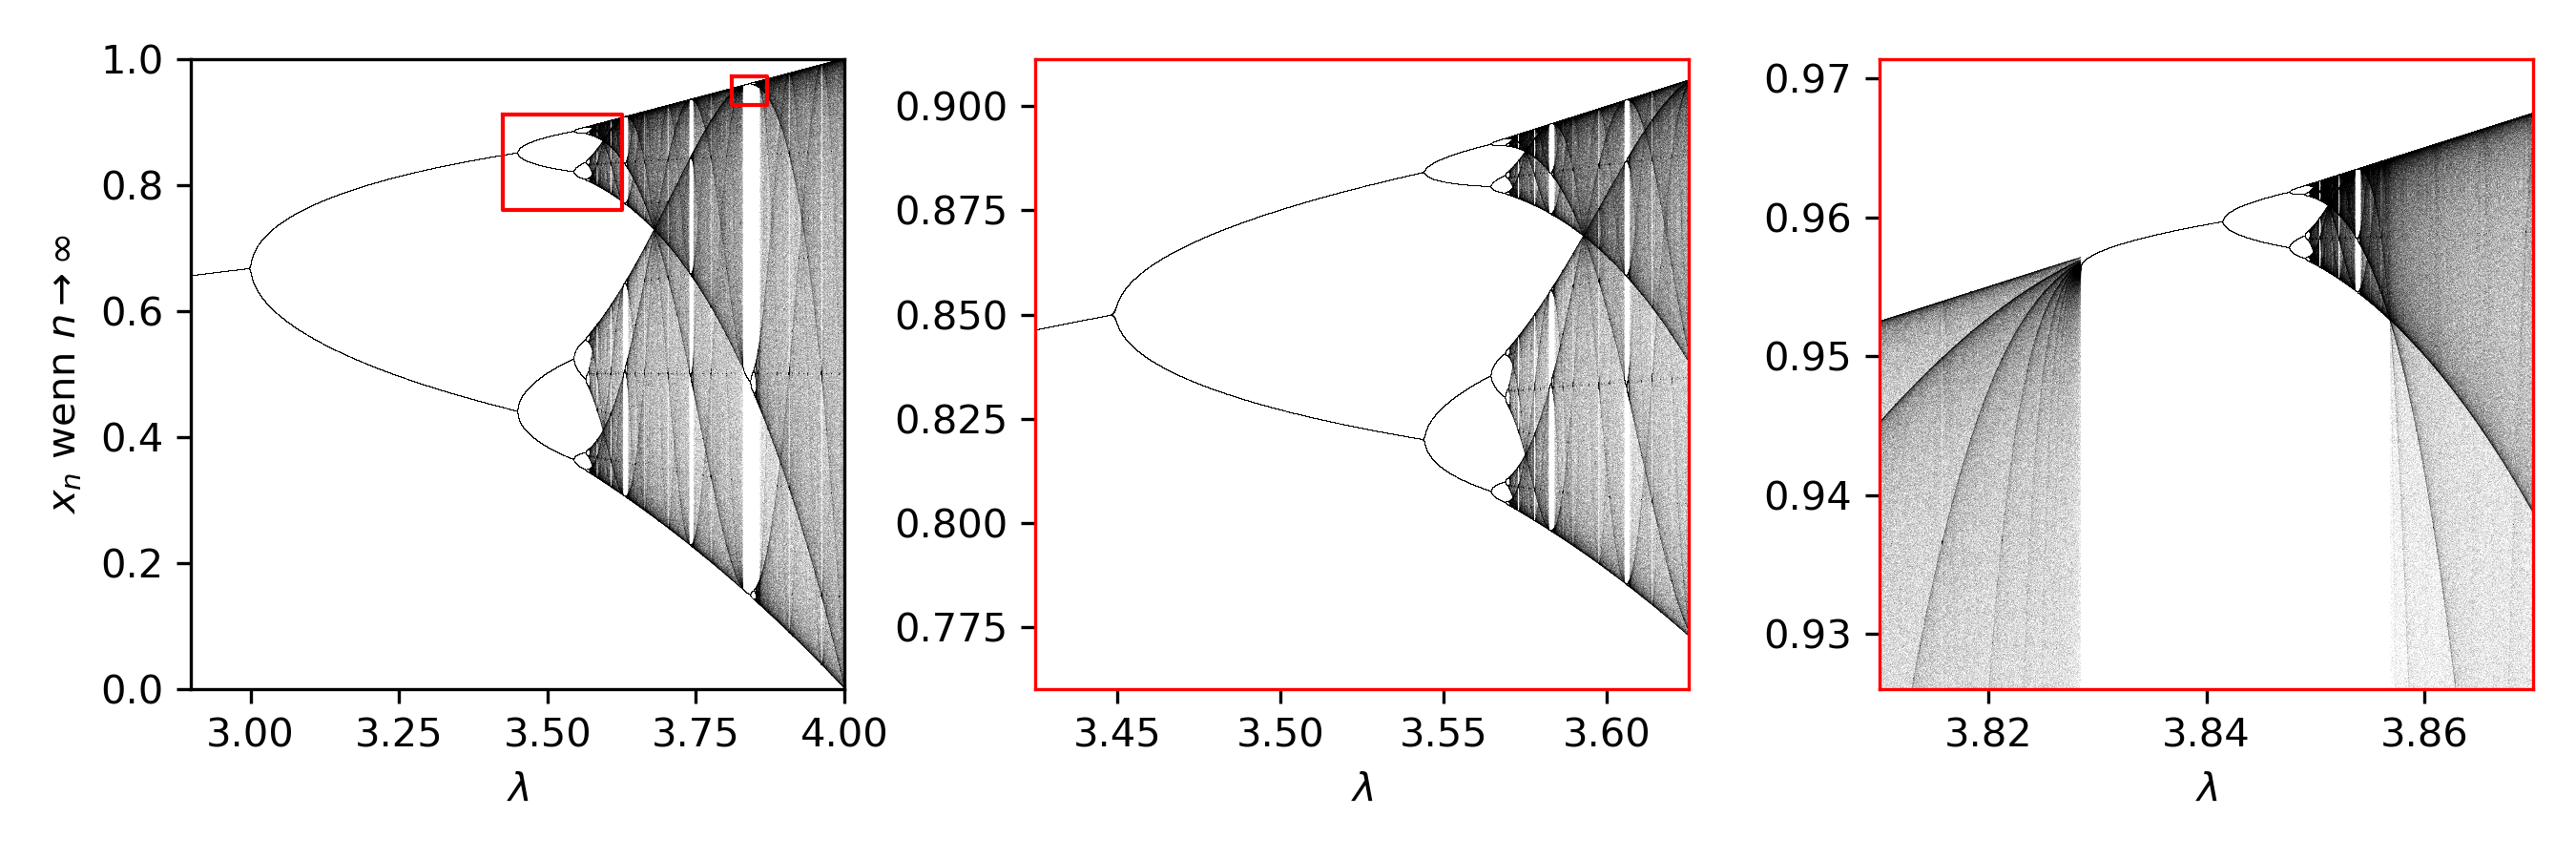
\includegraphics[width=\linewidth]{papers/logistic/figures/map_zoom.png}
    \caption{
        Das Bifurkationsdiagramm ist ein Fraktal.
        Die mittlere Grafik verdeutlicht mit einem Zoom 
        bei $\lambda = 3.525$ die Selbstänhlichkeit. 
        Auf der rechten Grafik sieht man mit einem
        Zoom bei $\lambda = 3.84$, dass sich immer
        wieder das selbe Muster finden lässt.
    }
    \label{fig:map_zoom}
\end{figure}

Des weiteren ist auf dem Bifurkationsdiagramm zu sehen,
dass für jede weitere Periodenverdoppelung eine geringere
Erhöhung von $\lambda$ notwendig ist.
Diese rapide zunehmende Dichte der Periodenverdoppelungen führt dazu, 
dass wenn $\lambda$ den Wert $\approx 3.57$ überschreitet, 
die Verdoppelungen aufhören und $x_n$ nicht mehr oszilliert. 
Stattdessen nimmt $x_n$ nur noch scheinbar 
willkürliche Werte in bestimmten Bereichen an, 
man spricht vom Chaos.
\index{Chaos}
Interessanterweise gibt es aber auch für Werte von 
$\lambda \gtrapprox 3.57$ wieder gewissen Bereiche,
wo wieder periodisches Verhalten auftritt. 
Ein Beispiel für einen solchen Bereich sieht man
gut in Abbildung \ref{fig:map_zoom} bei 
$\lambda \approx 3.83$. 
Dort gibt es zuerst eine Dreier-Periode, 
dann wieder die Periodenverdoppelungen, 
wobei die Dichte der Verdoppelungen
wieder rapide zunimmt.
Schliesslich bricht wieder das Chaos aus bei 
$\lambda \approx 3.85$.

%
% loesung.tex -- Beispiel-File für die Beschreibung der Loesung
%
% (c) 2020 Prof Dr Andreas Müller, Hochschule Rapperswil
%
\section{Stabilität der logistischen Gleichung
\label{logistic:section:stabil}}
\rhead{Stabilität der logistischen Gleichung}

In den bisherigen Grafiken ist leider nicht ersichtlich, 
warum die logistische Gleichung dieses Iterationsverhalten aufweist. 
Glücklicherweise kennen wir aber aus dem Kapitel 
\ref{buch:section:instabilitaet}
bereits Werkzeuge zur Stabilitätsbetrachtung für
das Iterieren von Funktionen. 
\index{Stabilität}%
Diese können wir jetzt einsetzen, damit wir dieses
Verhalten besser verstehen können. 

Kurze Auffrischung: Beim Iterieren einer Funktion
gibt es manchmal Fixpunkte. 
\index{Fixpunkte}%
Jeder Fixpunkt muss die Bedingung
$f(x^*)=x^*$ erfüllen, das heisst wenn man die Funktion
mit diesem Wert iteriert. passiert gar nichts, weil
immer wieder der gleiche Wert herauskommt. 
Grafisch sind diese Punkte die Schnittpunkte
vom Funktionsplot mit der 45°-Geraden durch den Ursprung.  
Zusätzlich gibt es die Stabilitätsbedingung 
$|f'(x^*)| < 1$. 
Wenn diese erfüllt ist, handelt es sich um einen
stabilen Fixpunkt. 
Er hat eine ``anziehende'' Wirkung. 
Grafisch sieht man das am Winkel der Tangente in den
Fixpunkten von $f(x)$, welcher zwischen +45° und -45° sein muss.

Wir können nun auf das uns bereits bekannte Spinnwebdiagramm
zurückgreifen, um grafisch diese Fixpunkte zu finden.
\index{Spinnwebdiagramm}%
Beim Betrachten der logistischen Gleichung 
$f(x) = \lambda x (1-x)$ sehen wir, 
dass es sich dabei eigentlich nur um eine Parabel mit 
den Nullstellen $0$ und $1$ handelt. 
Der Faktor $\lambda$ bestimmt die Öffnung der Parabel.  

Abbildung \ref{fig:web_1} zeigt nun das Spinnwebdiagramm,
welches wir beim Iterieren der logistischen Gleichung erhalten.  
Auf der linken Grafik mit $\lambda = 0.75$ sehen wir,
dass $x_n$ gegen den Fixpunkt bei $0$ konvergiert. 
Dies war bereits in Abbildung \ref{fig:pop_logistic} ersichtlich,
hier sehen wir aber zusätzlich noch, dass $x_n$ eben gegen
diesen Punkt konvergiert, weil es sich dabei um einen
stabilen Fixpunkt handelt.  
Auf der mittleren Grafik mit $\lambda = 1.8$ ist nun für den
Fixpunkt im Ursprung die Stabilitätsbedingung nicht
mehr erfüllt. 
Dafür ist sie jetzt für den zweiten Fixpunkt erfüllt, 
was dazu führt, dass die Funktion beim Iterieren gegen 
diesen Wert konvergiert.  
Auf der rechten Grafik mit $\lambda = 2.8$ ist wieder der  
zweite Fixpunkt stabil, hier ``umkreist'' die Linie aber
den Fixpunkt und konvergiert langsam gegen ihn. 
Auf Abbildung \ref{fig:pop_logistic} hat sich dieses Verhalten
als ``Einschwingen'' geäussert.
\index{Einschwingen}%
\begin{figure}[h!]
    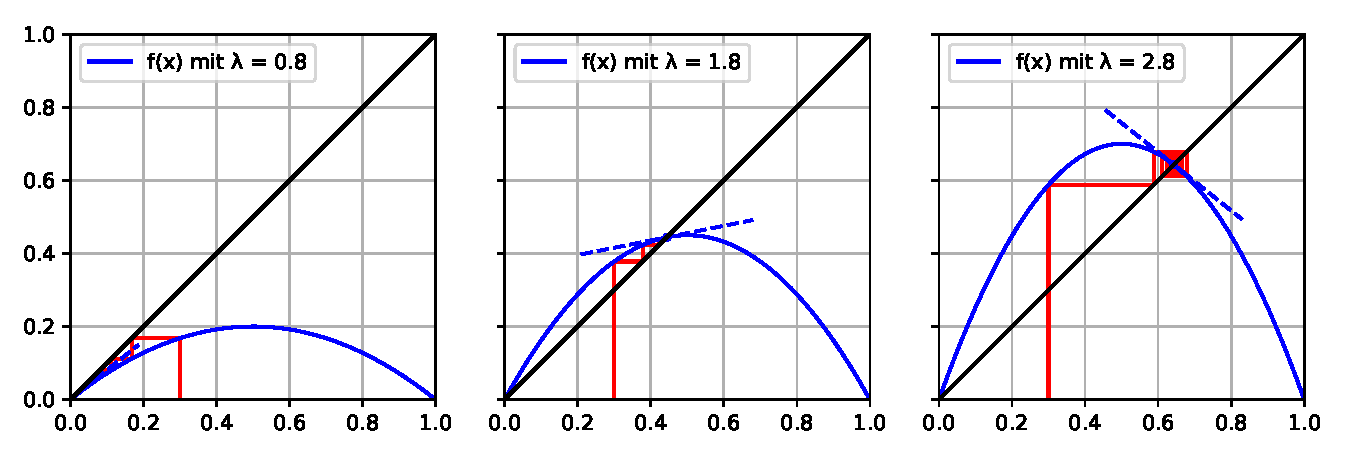
\includegraphics[width=\linewidth]{papers/logistic/figures/web_1.pdf}
    \caption{
        Spinnwebplot ohne Oszillation.
        Für alle drei Werte von $\lambda$ gibt es 
        einen stabilen Fixpunkt. 
        Auf der rechten Grafik mit $\lambda = 2.8$
        ist sichtbar wie $x_n$ 
        zuerst über- und dann langsam einschwingt.
    }
    \label{fig:web_1}
\end{figure}
\begin{figure}[h!]
    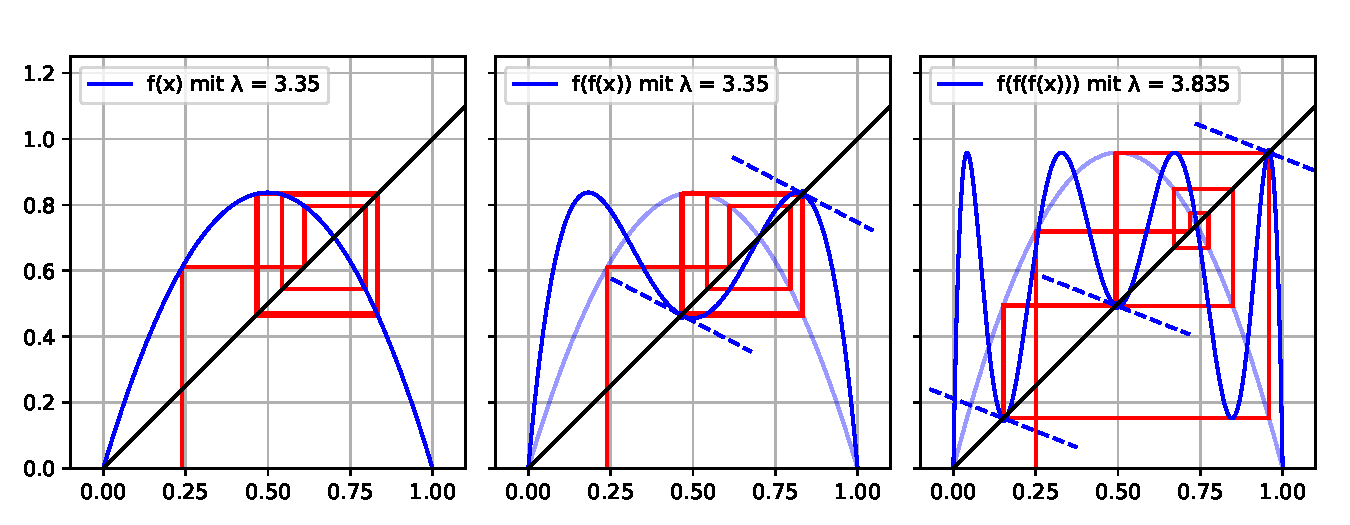
\includegraphics[width=\linewidth]{papers/logistic/figures/web_2.pdf}
    \caption{
        Spinnwebplot mit oszillierenden $x_n$. 
        Die mittlere Grafik zeigt, wie 
        die Verschachtelung $f(f(x))$ mit 
        $\lambda = 3.35$ zwei
        stabile Fixpunkte hervorbringt und erklärt
        damit die Oszillation zwischen
        den zwei Punkten in der linken Grafik.
        In der rechten Grafik zeigt eine weitere 
        Verschachtelung zu $f(f(f(x)))$
        mit $\lambda = 3.835$ 
        drei stabile Fixpunkte, was
        die entsprechende Dreier-Periode aus dem 
        Bifurkationsdiagramm (Abbildung \ref{fig:map_1})
        erklärt. 
    }
    \label{fig:web_2}
\end{figure}

Nun haben wir eine gute Erklärung für das Iterationsverhalten
der logistischen Gleichung für $0 < \lambda < 3$. 
Aber was passiert nun, wenn $\lambda > 3$ wird,
wo es beginnt zwischen mehreren Punkten zu oszillieren?
Wenn wir die Stabilitätsbedingung $|f'(x^*)| < 1$
für Fixpunkte von $f(x)$ mit $\lambda > 3$ anwenden sehen wir,
dass für eine einzelne Iteration der logistischen 
Gleichung kein stabiler Fixpunkte mehr existiert. 
Wenn wir jetzt aber zwei Iterationen der logistischen
Gleichung machen, also 
$f(f(x))$ wobei $f(x)=\lambda x (1-x)$,
dann bekommen wir ein Polynom vierten Grades:
\begin{equation}
    f(f(x))
    =
    \lambda [\lambda x (1-x)] (1-[\lambda x (1-x)])
    =
    \lambda^2 x (1-x) (\lambda x^2 - \lambda x + 1).
\end{equation}
Diese neue Funktion bringt mit der 45°-Geraden 
neue Schnittpunkte und damit auch neue Fixpunkte mit sich.
Tatsächlich finden wir unter diesen neuen Fixpunkten 
auch solche, welche die Stabilitätsbedingung erfüllen für
Werte von $\lambda > 3$.

Auch das wollen wir uns nochmal grafisch mit
Abbildung \ref{fig:web_2} veranschaulichen.  
Auf der linken Grafik ist das Spinnwebdiagramm der 
logistischen Gleichung mit $\lambda = 3.35$ und
$f(x)$ abgebildet. 
Offenbar gibt es eine Oszillation zwischen zwei Punkten.
Jedoch ist nicht sichtbar, warum das so sein sollte,
es gibt da keinen stabilen Fixpunkt zu sehen.
Auf der mittleren Grafik ist nun nochmal das gleiche
Spinnwebdiagramm, jetzt ist aber zusätzlich noch
die verschachtelte Funktion $f(f(x))$ sichtbar.
Darauf wird deutlich, warum die Oszillation eben genau 
zwischen diesen beiden Punkten entsteht. 
Es handelt sich dabei um zwei Fixpunkte, welche erst 
mit der Verschachtelung von $f(x)$ sichtbar werden.
\index{Verschachtelung}%
Würde man $\lambda$ nun weiter erhöhen, würden auch
diese beiden Fixpunkte wieder instabil werden,
dafür vier neue stabile Fixpunkte bei einer erneuten
Verschachtelung erscheinen, 
also bei $f(f(f(f(x))))$. 
Das geht so weiter bis zum Anfang des Chaos, wo
es keine stabilen Fixpunkte mehr gibt. 
Wenn wir aber weiter durch das Chaos gehen gibt es, 
wie in Kapitel \ref{logistic:section:analyse}
zu sehen war, immer wieder diese kleinen Fenster,
wo $x_n$ wieder periodisch wird. 
Da gibt es zum Beispiel bei
$\lambda \approx 3.835$ eine Dreier-Periode,
was vermuten lässt, dass für diesen Wert
von $\lambda$ durch die dreifache Verschachtelung
von $f(x)$ wieder drei stabile Fixpunkte entstehen.
Tatsächlich gibt es, wie auf der rechten Grafik 
in Abbildung \ref{fig:web_2} zu sehen ist,
durch $f(f(f(x)))$ und $\lambda = 3.835$ drei stabile Fixpunkte. 


\FloatBarrier

%
% problemstellung.tex -- Beispiel-File für die Beschreibung des Problems
%
% (c) 2020 Prof Dr Andreas Müller, Hochschule Rapperswil
%
\section{Beispiele von verwandten Funktionen
\label{logistic:section:beispiele}}
\rhead{Beispiele von verwandten Funktionen}
\begin{figure}[h!]
    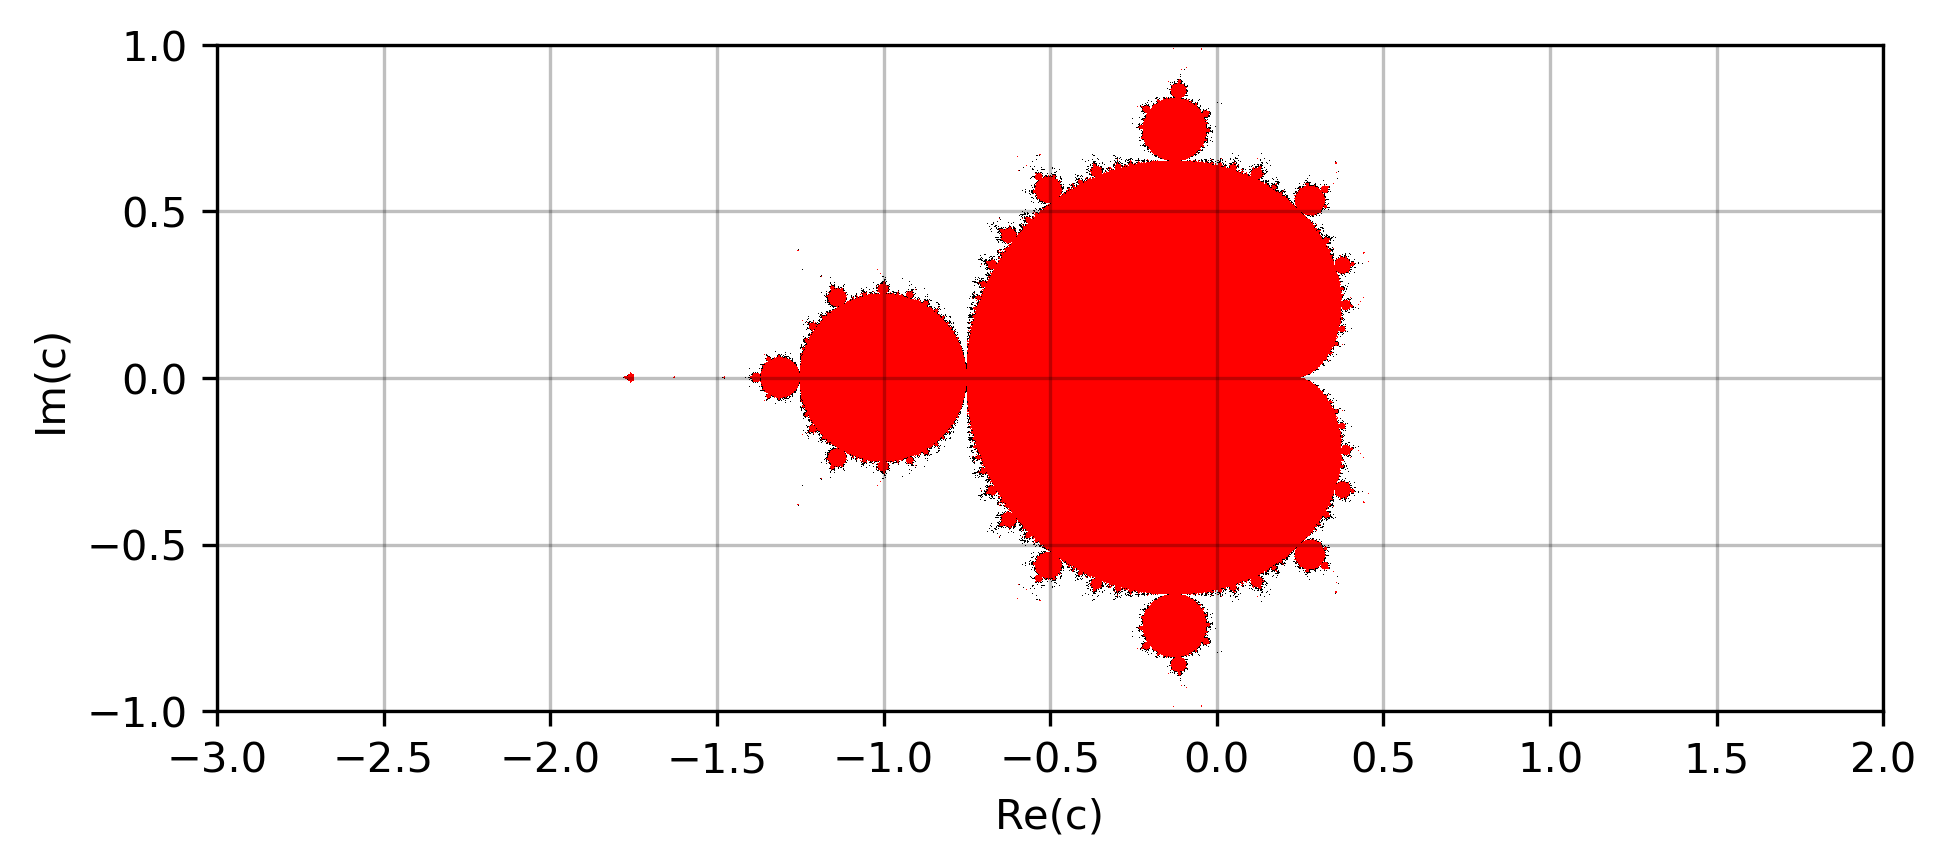
\includegraphics[width=\linewidth]{papers/logistic/figures/mandel.png}
    \caption{Mandelbrotmenge}
    \label{fig:mandel_2d}
\end{figure}
%\FloatBarrier
\subsection{Mandelbrotmenge}
\index{Mandelbrotmenge}%
\begin{figure}
    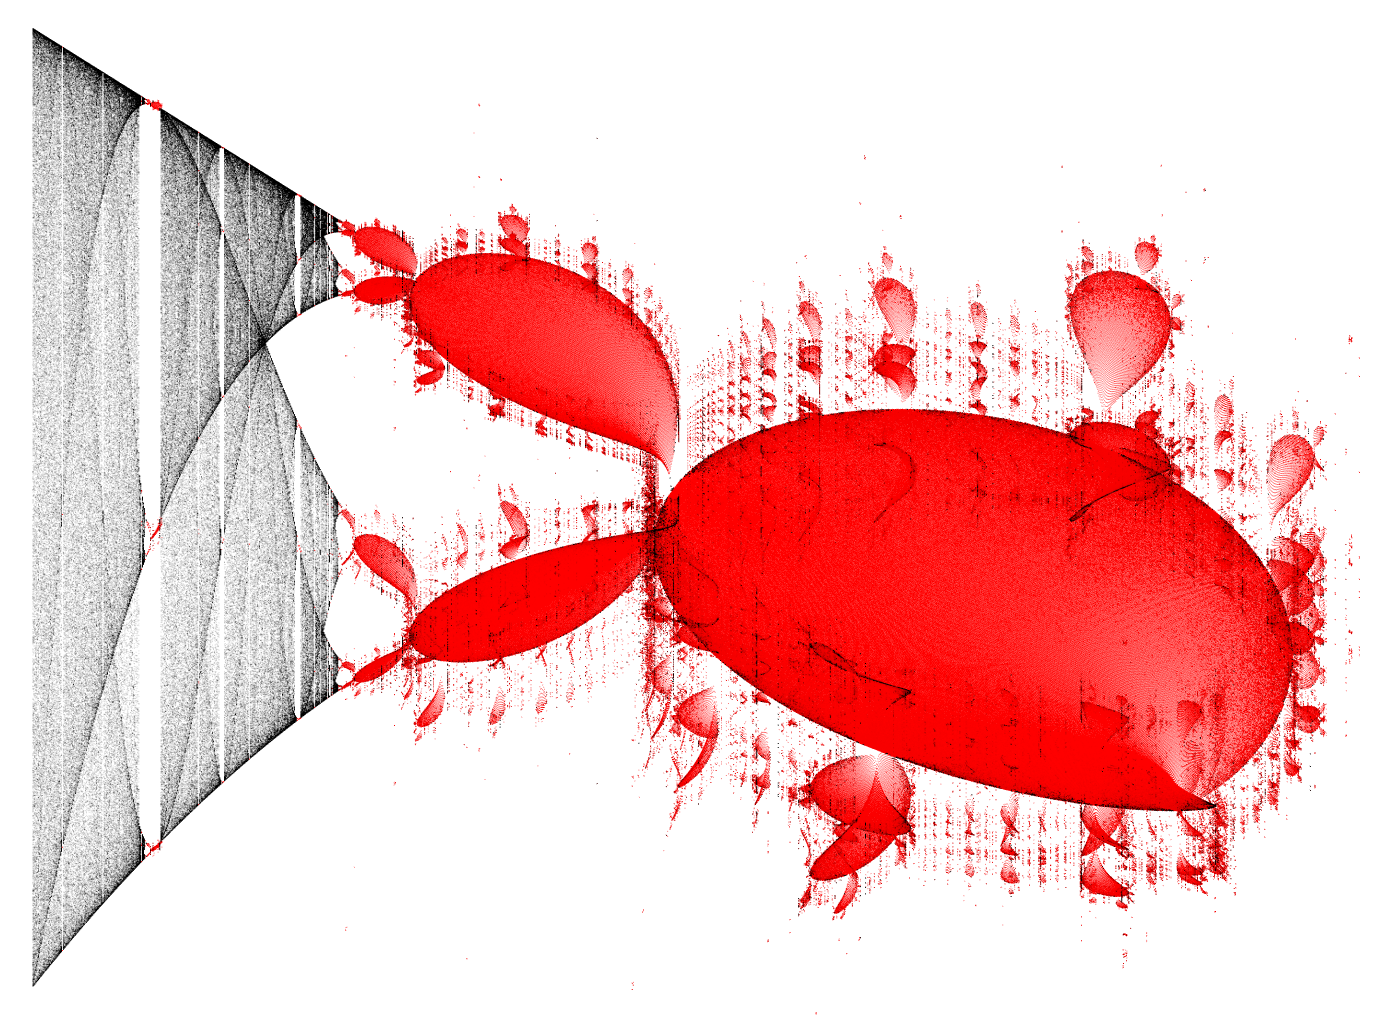
\includegraphics[width=\linewidth]{papers/logistic/figures/mandel_3d.png}
    \caption{
        Dreidimensionales Bifurkationsdiagramm der Mandelbrotmenge.
        Das Bild wird aus einem flachen Winkel 
        leicht von oben angeschaut. 
        Die horizontale Ebene repräsentiert die
        Werte von $c$, siehe Abbildung \ref{fig:mandel_2d}
        zum Vergleich.
        Die vertikale Achse zeigt
        die Werte, die $\Re(z_n)$ annimmt wenn 
        $n \rightarrow \infty$.
        Rote Farbe bedeutet, dass $\Re(z_n)$ eine
        endliche Periode hat, schwarze Farbe bedeutet
        chaotisches Verhalten. 
        Besonders interessant ist das Gebilde auf der 
        linken Seite, das dem Bifurkationsdiagramm
        der logistischen Gleichung sehr änhlich sieht.
    }
    \label{fig:mandel_3d}
\end{figure}
In Kapitel \ref{logistic:section:analyse} 
haben wir bereits gesehen, 
dass das Bifurkationsdiagramm der logistischen Gleichung
ein Fraktal ist. 
Eines der bekanntesten Fraktale ist die Mandelbrotmenge,
deren Gleichung der logistischen Gleichung sehr ähnlich ist. 
Die Iterationsgleichung der Mandelbrotmenge lautet
\begin{equation}
    z_{n+1} = z_n^2 + c\text{,}
    \label{eq:mandelbrot}
\end{equation}
wobei $z_n$ und $c$ komplexe Zahlen sind und 
der Einfachkeit halber $z_0 = 0$ gesetzt werden kann.
Zum Vergleich, die logistische Gleichung hat ausmultipliziert
die Form $x_{n+1} = -\lambda x_n^2 +\lambda x_n$. 
Wie bei der logistischen Gleichung gibt es auch
bei der Gleichung der Mandelbrotmenge wieder bestimmte
Werte von $c$, bei der $z_n$ entweder 
divergiert, 
konvergiert, 
oszilliert 
oder in chaotisches Verhalten ausbricht. 
Jeder Wert von $c$, für den $z_n$ nicht 
divergiert, ist Teil der Mandelbrotmenge. 
Nun können wir, ähnlich wie schon beim 
Bifurkationsdiagramm der logistischen Gleichung, auf der
komplexen Ebene für jeden Wert von $c$ das Verhalten
der Gleichung der Mandelbrotmenge darstellen. 
Dazu färben wir den Bereich, in dem $z_n$ 
nicht divergiert, rot ein.
Damit sehen wir in Abbildung \ref{fig:mandel_2d}
die Mandelbrotmenge. 
Auf dieser zweidimensionalen Darstellung ist jedoch nicht zu sehen, 
welche Werte $z_n$ annimmt.
Darum nehmen wir jetzt die dritte Dimension zur Hilfe um,
wie schon beim Bifurkationsdiagramm der logistischen Gleichung,
auf der vertikalen Achse darzustellen, 
auf welchem Wert sich der Wert von $z_n$ schlussendlich einpendelt.
Oder eben auch nicht, wenn es oszilliert oder sogar
chaotisch wird. 
Da wir nur drei Dimensionen zur Verfügung haben,
beschränken uns dabei auf den Realteil von $z_n$. 
Das Ergebnis davon ist in Abbildung 
\ref{fig:mandel_3d}
zu sehen. 
Die Farben geben Auskunft über die Periodizität des 
jeweiligen Punktes. 
Rote Farbe bedeutet, dass $\Re(z_n)$
für den jeweiligen Wert von $c$ eine endliche 
Periode hat. 
Schwarz bedeutet chaotisches Verhalten 
oder möglicherweise auch,
dass die Periode so gross ist, dass der Computer
sie bei der Berechnung nicht als endlich erkannt hat.
Auf der reellen Achse ist deutlich ein Gebilde zu sehen,
welches dem Bifurkationsdiagramm der logistischen
Gleichung sehr ähnlich sieht. 
Ebenfalls zu sehen ist, dass die kreisförmigen
``Platformen'' sich regelmässig verdoppeln, weil
$\Re(z_n)$ zwischen immer mehr Werten hin und her oszilliert.

\subsection{Universelle Eigenschaft}
\begin{figure}
    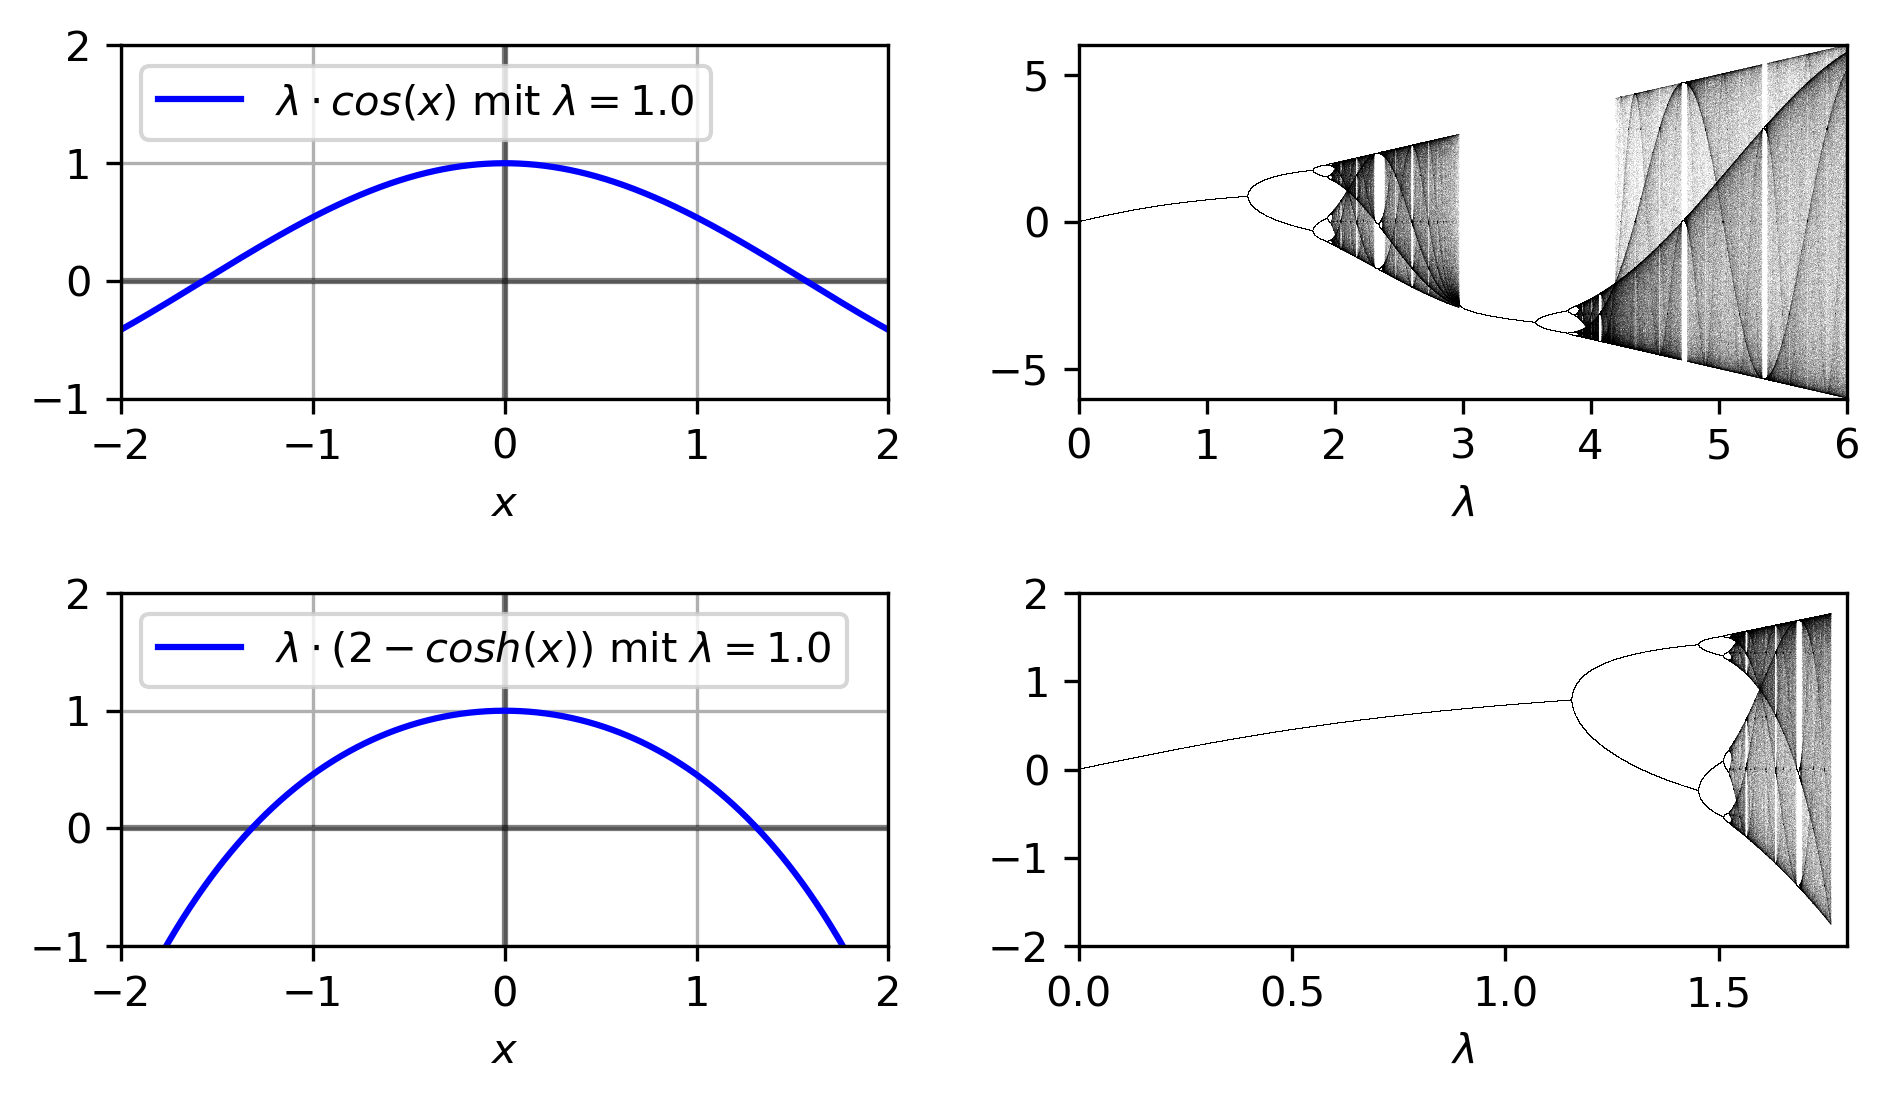
\includegraphics[width=\linewidth]{papers/logistic/figures/universal.png}
    \caption{
        Bifurkationsdiagramme von 
        $\lambda \cdot \cos(x)$
        und
        $\lambda \cdot (2 - \cosh(x))$.
        Links ist jeweils der Funktionsplot und
        rechts das dazugehörige Bifurkationsdiagramm. 
    }
    \label{fig:universal}
\end{figure}
\index{universelle Eigenschaft}%
Dieses Verhalten mit den Periodenverdoppelungen 
bis es schliesslich chaotisch wird und dann
immer wieder kurzen oszillierenden Fenstern im Chaos
ist keineswegs eine Eigenschaft, 
die nur die logistische Gleichung besitzt.
Man findet dieses Verhalten auch beim Iterieren 
von vielen anderen nichtlinearen Funktionen. 
Ein typisches Merkmal, 
an dem man Funktionen erkennt
die diese Eigenschaften aufweisen, 
sind ``Hügel'' im Funktionsplot.
Als Beispiel dazu sind in Abbildung \ref{fig:universal} links
die beiden Funktionen
$\lambda \cdot \cos(x)$
und
$\lambda \cdot (2 - \cosh(x))$
abgebildet.
Beide Funktionen haben, wie auch schon die Funktion
der logistischen Gleichung, einen Hügel. 
Rechts sind die Bifurkationsdiagramme dieser beiden
Funktionen abgebildet. 
Die Ähnlichkeiten zum Bifurkationsdiagramm der logistischen
Gleichung sind deutlich sichtbar. 
Besonders interessant wird es, wenn man
bei diesen Funktionen im Bifurkationsdiagramm 
die Periodenverdoppelungen genauer anschaut.
Denn wenn man das Verhältnis der Breite einer Periode
zur Breite der vorherigen Periode im Limit
anschaut, also 
$
    \lim_{n\to\infty}(\frac{\lambda_{n-1} - \lambda_{n-2}}{\lambda_n - \lambda_{n-1}})
$
wobei $\lambda_n$ der Wert von $\lambda$ bei der $n$-ten
Periodenverdoppelung ist,
dann kommt man auf die Zahl $\delta \approx 4.6692$.
Diese Zahl hat den Namen ``Feigenbaum-Konstante''.
Es ist irrelevant, welche Kaskade von Periodenverdoppelungen
\index{Kaskade von Periodenverdoppelungen}%
bei diesen Funktionen
gewählt wird, im Limit kommt schlussendlich immer diese Zahl heraus. 
Die Feigenbaum-Konstante findet man auf die genau gleiche Art 
\index{Feigenbaum-Konstante}%
auch in der logistischen Gleichung und in vielen anderen
Funktionen, die einen einzelnen ``Hügel'' haben, wieder.
Dadurch haben alle diese Funktionen durch die 
Feigenbaum-Konstante eine universale Eigenschaft.
Es ist überhaupt nicht offentsichtlich warum das so
sein sollte und es hat Mitchell Feigenbaum, 
\index{Feigenbaum, Mitchell}%
den Entdecker dieser Konstante, und andere Mathematiker 
viel Arbeit gekostet, diese Eigenschaft zu erforschen. 

Abschliessend können wir so aus diesen Erkenntnissen direkt 
noch etwas für die weitere Numerik mitnehmen.
Offenbar können sich Funktionen beim Iterieren sehr 
unerwartet verhalten. 
Gerade in der Numerik bauen viele Verfahren
auf iterativen Algorithmen auf. 
Deswegen schadet es sicherlich nicht,
wenn man sich bewusst ist, dass beim Iterieren von
scheinbar einfachen Funktionen so ein ``wildes'' 
Verhalten enstehen kann. 


\printbibliography[heading=subbibliography]
\end{refsection}
